\chapter{Numerical Algebra}\label{ch:numerical_algebra}

\section{A Root Finding Game}
Let's play a game!
\begin{problem}\label{prob:bisection_game}
    Find a partner in the room to play a two-person game.  Choose someone to go first and
    follow these steps to play.
    \begin{description}
        \item[Step \#1:] The first player secretly chooses a positive real number. For
            simplicity let's choose something less than 100.
        \item[Step \#2:] The first player chooses non-negative real numbers $a$ and $b$ so that the
            secret number is between $a$ and $b$.  
        \item[Step \#3:] The first player tells the second player ``{\it my number is between $a$
            and $b$}''.
        \item[Step \#4:] The second player makes a guess at the secret number.  We'll call
            that number $c$.
        \item[Step \#5:] The first player responds with one of the following three
            responses.
            \begin{itemize}
                \item If $c$ is within $0.01$ of the secret number then say\\ ``{\it you win!}''
                \item If the secret number is between $a$ and $c$ then say\\ ``{\it the secret
                number is between $a$ and $c$}.''
                \item If the secret number is between $c$ and $b$ then say\\ ``{\it the secret
                number is between $c$ and $b$}.''
            \end{itemize}
        \item[Step \#6:] Repeat steps 4 and 5 until the second player guesses the secret
            number to within $0.01$ or you have repeated more than 20 times. The second
            player wins if he/she guesses the number in 20 or fewer steps.
    \end{description}
\end{problem}

\begin{problem}
    Discuss with your partner what the optimal strategy for the second player is for the
    game in Problem \ref{prob:bisection_game}.
\end{problem}

\begin{problem}
    Write \ProgLang code so you can play the game from Problem
    \ref{prob:bisection_game} against the computer.  
    The following incomplete code should get you started.  Fill in the missing pieces of
    the code and play the game several times to be sure that it works.  What strategy do
    you find yourself using to play the game? 
    \ifnum\Python=0
\begin{lstlisting}
%% Secret Number Guesser Game
clear; clc; format compact;
secret = 100*rand(1,1); % random secret number between 0 and 100
tolerance = 0.01;
a = randi(floor(secret),1); % initial lower bound integer below the secret
b = randi( [ceil(secret),101] , 1); % initial upper bound integer above the secret
guess = 1000; % dummy initial value for the guess
n = 1; % initialize the game counter
while abs( secret - c ) > tolerance && n < 20
    fprintf('Guess number %g.\n',n)
    fprintf('The secret number is between %g and %g.\n',a,b)
    guess = input('What is your guess for the secret number? ');
    if abs( secret - guess ) < tolerance
        fprintf('Close enough!  The actual random number was %g. \n',secret) 
        break
    elseif guess < (secret-tolerance)
        ... % write appropriate code here in this case
    elseif guess > (secret+tolerance)
        ... % write appropriate code here in this case
    end
    n=n+1; % increment the game counter
end
\end{lstlisting}
\else
\begin{lstlisting}
from numpy import *
secret = 100*rand(1,1) # get the secret random number
secret = secret[0,0]
tolerance = 0.01

# initial lower bound integer below secret number
a = float(randint(low=0, high=floor(secret))) 
# initial lower bound integer below secret number
b = float(randint(low=ceil(secret),high=101))

guess = 1000 # initial guess
n = 1 # initialize the game counter
while abs( secret - guess ) > tolerance and n < 20:
    print('Guess Number',n)
    print('The secret number is between',a,' and ',b)
    guess = float(input('What is your guess for the secret number?'))
    if abs(secret - guess) < tolerance:
        print("Close enough!  The random number was",secret)
        break
    elif guess < (secret - tolerance):
        ... # write appropriate code here in this case
    elif guess > (secret + tolerance):
        ... # write appropriate code here in this case
    n += 1 # increment the game counter
\end{lstlisting}
\fi
\end{problem}



\newpage
\section{Introduction to Root Finding}
In this chapter we want to solve algebraic equations using a computer.  Consider the equation
$\ell(x) = r(x)$ (where $\ell$ and $r$ stand for left and right respectively).  To solve
this equation we can first rewrite it by subtracting the right-hand side from the left to
get
\[ \ell(x) - r(x) = 0. \]
For example, if we want to solve $3\sin(x) + 9 = x^2 - \cos(x)$ then this is the same as
solving $(3\sin(x) + 9 ) - (x^2 - \cos(x)) = 0$.  Hence, we can define a function $f(x)$
as $f(x)=\ell(x)-r(x)$
and observe that \underline{every} algebraic equation can be written as: ``if $f(x) = 0$,
find $x$''.  We illustrate this idea in Figure \ref{fig:initial_root_example}.  On the
left-hand side of Figure \ref{fig:initial_root_example} we see the solutions to the
equation $3\sin(x) + 9 = x^2 - \cos(x)$, and on the right-hand side of Figure
\ref{fig:initial_root_example} we see the solutions to the equation $\left( 3\sin(x)+9
\right) - \left( x^2 - \cos(x) \right) = 0$.  From the plots it is apparent that the two
equations have the same solutions: $x_1 \approx -2.55$ and $x_2 \approx 2.88$.

\begin{figure}[ht!]
    \begin{center}
        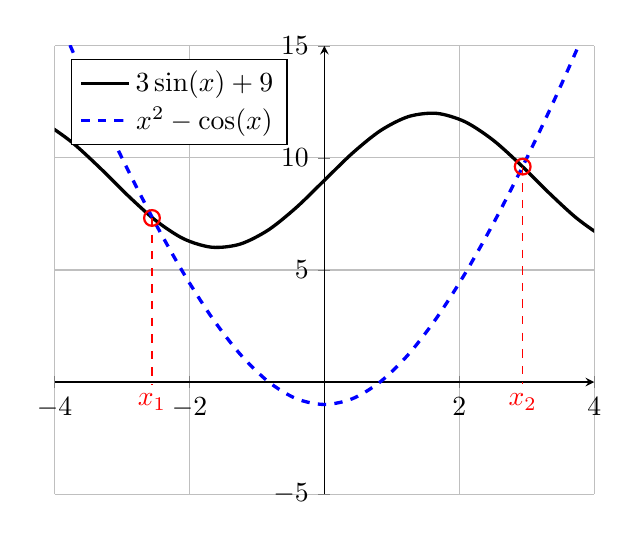
\begin{tikzpicture}
            \begin{axis}[axis lines=center, grid, xmin=-4, xmax=4, ymin=-5, ymax=15, legend
                pos=north west]
                \addplot[black, smooth, very thick] {3*sin(deg(x)) + 9};
                \addlegendentry{$3\sin(x) + 9$};
                \addplot[blue, smooth, dashed, very thick] {x^2 - cos(deg(x))};
                \addlegendentry{$x^2-\cos(x)$};
                \draw[thick, red] (axis cs:-2.556,7.32) circle(0.1cm);
                \draw[dashed, red] (axis cs:-2.556,7.32) -- (axis cs:-2.556,-0.1) node[anchor=north]{$x_1$};
                \draw[thick, red] (axis cs:2.94,9.61) circle(0.1cm);
                \draw[dashed, red] (axis cs:2.94,9.61) -- (axis cs:2.94,-0.1)
                node[anchor=north]{$x_2$};
            \end{axis}
        \end{tikzpicture}
        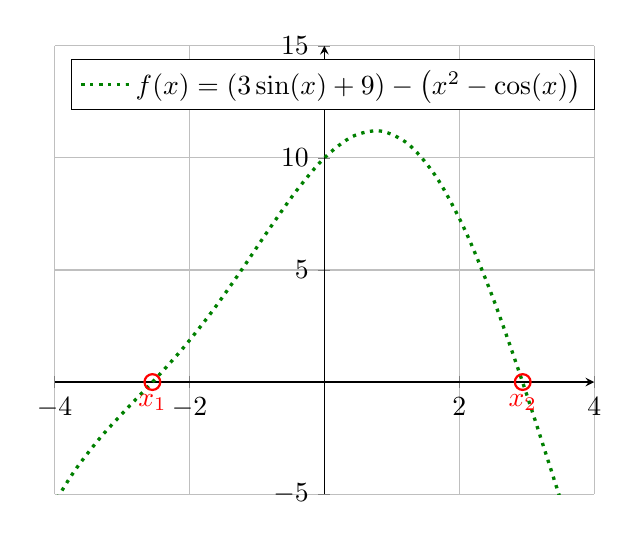
\begin{tikzpicture}
            \begin{axis}[axis lines=center, grid, xmin=-4, xmax=4, ymin=-5, ymax=15, legend
                pos=north west]
                \addplot[black!50!green, dotted, smooth, very thick] {3*sin(deg(x)) + 9 - x^2
                + cos(deg(x))};
                \addlegendentry{$f(x) = \left(3\sin(x) + 9\right) - \left( x^2-\cos(x)\right)$};
                \draw[thick, red] (axis cs:-2.55,0) circle(0.1cm);
                \draw[thick, red] (axis cs:-2.55,-0.1) node[anchor=north]{$x_1$};
                \draw[thick, red] (axis cs:2.94,0) circle(0.1cm);
                \draw[thick, red] (axis cs:2.94,-0.1) node[anchor=north]{$x_2$};
            \end{axis}
        \end{tikzpicture}
    \end{center}
    \caption{The left-hand plot shows two nonlinear functions, $\ell(x) = 3\sin(x) + 9$ and
        $r(x) = x^2 - \cos(x)$, with their intersection points marked. The right-hand plot
    shows the equivalent problem formed by solving $\ell(x) - r(x) = 0$.}
    \label{fig:initial_root_example}
\end{figure}

We now have one way to view every algebraic equation-solving problem.  As we'll see in
this chapter, if $f(x)$ has certain properties then different numerical techniques for
solving the equation will apply -- and some will be much faster and more accurate than
others. The following sections give several different techniques for solving algebraic
equations of the form $f(x) = 0$.

\begin{problem}
    With a partner make three different plots just like Figure
    \ref{fig:initial_root_example}.  Do so by picking an algebraic root-finding problem,
    plotting the left and right sides on top of each other (for the left-hand plot) and
    then plotting the difference between the left and right sides of your equation (for
    the right-hand plot).  Visually verify that the intersections you see on the left-hand
    plot and the same as the roots on the right-hand plot each time.
\end{problem}

\newpage
\section{The Bisection Method}
We'll start the mathematical discussion with a theorem from Calculus.
\begin{thm}[The Intermediate Value Theorem (IVT)]
    If $f(x)$ is a continuous function on the closed interval $[a,b]$ and $y_*$ lies between
    $f(a)$ and $f(b)$, then there exists some point $x_* \in [a,b]$ such that $f(x_*) = y_*$.
    \label{thm:IVT}
\end{thm}


\begin{problem}
    Draw a picture of what the intermediate value theorem says graphically.
\end{problem}
\solution{
Draw a continuous function that crosses the line $y=y_*$ on the interval $[a,b]$.
}

\begin{problem}
    If $y_*=0$ the intermediate value theorem gives us important information about solving
    equations.  What does it tell us?
\end{problem}
\solution{
If $y_*=0$ and $f(x)$ is continuous then we know that there is a solution to the algebraic
equation $f(x) = 0$.
}

\begin{cor}
    If $f(x)$ is a continuous function on the closed interval $[a,b]$ and if $f(a)$ and $f(b)$ have opposite
    signs then from the Intermediate Value Theorem we know that there exists some point
    $x_* \in [a,b]$ such that \underline{\hspace{1in}}.
\end{cor}

Theorem \ref{thm:IVT} and its corollary are {\it existence theorems} in the sense that
they tell us that some point exists.  The annoying thing about mathematical existence
theorems is that they typically don't tell us {\it how} to find the point that is guaranteed to
exist -- annoying.  Let's play a game that might at least tell us how to find the root.
% The following algorithm, known as the Bisection Method, uses the Intermediate
% Value Theorem to systematically approximate the point $x_*$ to solve the algebraic
% equation $f(x_*) =
% 0$.

% \begin{problem}
%     Discussion: What does the game from Problem \ref{prob:bisection_game} have in common
%     with the Intermediate Value Theorem and its corollary?  Use your optimal strategy from
%     the game along with the corollary to the IVT to propose a strategy to find roots of a
%     continuous function.  Write psuedo-code for your solution strategy.
% \end{problem}

\begin{problem}
    Let's make a modification to the game from Problem \ref{prob:bisection_game}.  In
    groups of 2 follow these rules to play a root-finding game.
    \begin{description}
        \item[Step \#1:] Player 1 chooses a \underline{continuous} function $f(x)$ that
            has a root somewhere on the real line.  
        \item[Step \#2:] Player 1 chooses real numbers $x=a$ and $x=b$ so that the root of
            $f(x)$ is between those values.
        \item[Step \#3:] Player 1 tells Player 2 {\it ``the root of my function is between
            $a$ and $b$''}.
        \item[Step \#4:] Player 2 makes a guess of the root.  We'll call that number $m$.
        \item[Step \#5:] Player 1 reponds with one of the following three responses.
            \begin{itemize}
                \item If $m$ is within $0.01$ of the root of $f(x)$ then say \\ {\it ``you
                    win!''}
                \item If the root of $f(x)$ is between $a$ and $m$ then say \\ {\it ``the
                    root is between $a$ and $m$''}
                \item If the root of $f(x)$ is between $m$ and $b$ then say \\ {\it ``the
                    root is between $m$ and $b$''}
            \end{itemize}
        \item[Step \#6:] Repeat steps 4 and 5 until Player 2 has a reasonable guess of the
            root or until you have repeated these steps more than 20 times.
    \end{description}
\end{problem}

\begin{problem}
    Consider the game that you played in the previous problem.
    \begin{enumerate}
        \item[(a)] Where was the Intermediate Value Theorem used in the game?  Which
            player was using it and why were they using it?
        \item[(b)] Why was it important that the function $f(x)$ was continuous in this
            game?
        \item[(c)] Propose an optimal strategy for finding the root with the information
            given.
        \item[(d)] Write an outline of computer code (called pseudo-code) that will play
            this game with a given function and given initial values of $a$ and $b$.
    \end{enumerate}
\end{problem}

The pseudo-code that you wrote in the previous problem is likely very similar to the
``bisection method'' for finding roots of an algebraic function.  In the following
algorithm there are several questions you need to answer.
\begin{algorithm}[The Bisection Method]
    Assume that $f(x)$ is continuous on the closed interval $[a,b]$. To make approximations of
    the solutions to the equation $f(x) = 0$, do the following:
    \begin{enumerate}
        \item Check to see if $f(a)$ and $f(b)$ have opposite signs.  You can do this
            taking the product of $f(a)$ and $f(b)$.
            \begin{itemize}
                \item If $f(a)$ and $f(b)$ have different signs then what does the IVT
                    tell you?
                \item If $f(a)$ and $f(b)$ have the same sign then what does the IVT not
                    tell you? What should you do in this case?
                \item Why does the product of $f(a)$ and $f(b)$ tell us something about
                    the signs of the two numbers?
            \end{itemize}
            
        \item Compute the midpoint of the closed interval, $m=\frac{a+b}{2}$, and evaluate
            $f(m)$. 
            \begin{itemize}
                \item Will $m$ always be a better guess of the root than $a$ or $b$?  Why?
                \item What should you do here if $f(m)$ is really close to zero?
            \end{itemize}
        \item Compare the signs of $f(a)$ vs $f(m)$ and $f(b)$ vs $f(m)$.  
            \begin{itemize}
                \item What do you do if $f(a)$ and $f(m)$ have opposite signs?
                \item What do you do if $f(m)$ and $f(b)$ have opposite signs?
            \end{itemize}

        \item Repeat steps 2 and 3 and stop when $f(m)$ is {\it close enough} to zero.
    \end{enumerate}
\end{algorithm}

\begin{problem}
    Draw a picture illustrating what the Bisection Method does to approximate solutions to
    the algebraic equation $f(x) = 0$.
\end{problem}


\begin{problem}
    We want to write a \ProgLang function for the Bisection Method.  Instead of jumping
    straight into the code we should ALWAYS write pseudo-code first.  It is often helpful
    to write pseudo-code as comments in your \ProgLang file.  Use the template below to
    complete your pseudo-code.
    \ifnum\Python=0
\begin{lstlisting}
function root = Bisection(f , a , b , tol)
% The input parameters are
% f is an anonymous function handle
% a is the lower guess
% b is the upper guess
% tol is an optional tolerance for the accuracy of the root

% if the user doesn't define a tolerance we need code to create a default

% check that there is a root between a and b
% if not we should return an error and break the code

% next calculate the midpoint m = (a+b)/2

% start a while loop
    % in the while loop we need an if statement
    % if ...
    % elseif ...
    % elseif ...

    % we should check that the while loop isn't running away

% end the while loop
% define the root
\end{lstlisting}
\else
\begin{lstlisting}
def Bisection(f , a , b , tol):
# The input parameters are
# f is a function
# a is the lower guess
# b is the upper guess
# tol is an optional tolerance for the accuracy of the root

# if the user doesn't define a tolerance we need code to create a default

# check that there is a root between a and b
# if not we should return an error and break the code

# next calculate the midpoint m = (a+b)/2

# start a while loop
#   # in the while loop we need an if statement
#   # if ...
#   # elif ...
#   # elif ...

#   # we should check that the while loop isn't running away

# end the while loop
# define and return the root
\end{lstlisting}
\fi
\end{problem}


\begin{problem}
    Now use the pseudo-code as structure to complete a \ProgLang function for the Bisection
    Method.  Also write a test script that verifies that your function works properly. Be
    sure that it can take an anonymous function handle as an input along with an initial
    lower bound, an initial upper bound, and an optional error tolerance. The output
    should be only 1 single number: the root.\\
    \ifnum\Python=0 \mcode{function root=Bisection(f , a , b , tol)} 
    \else
    \mcode{def Bisection(f , a , b , tol):}
    \fi
\end{problem}

\begin{problem}
    Test your Bisection Method code on the following algebraic equations.
    \begin{enumerate}
        \item $x^2 - 2 = 0$ on $x \in [0,2]$ \solution{$\sqrt{2} \approx 1.414$}
        \item $\sin(x) + x^2 = 2\ln(x) + 5$ on $x \in [0,5]$ (be careful! make a plot
            first) \solution{$0.0860$ and $2.4953$ }
        \item $(5-x)e^{x}=5$ on $x \in [0,5]$\solution{$4.9651$}
    \end{enumerate}
\end{problem}


\begin{problem}
    Let $f(x)$ be a continuous function on the interval $[a,b]$ and assume that $f(a)
    \cdot f(b) <0$.  A reoccurring theme in Numerical Analysis is to approximate some
    mathematical thing to within some tolerance.  For example, if we want to approximate the solution to the equation $f(x)=0$ to
    within $\delta$ with the bisection method, we should be able to figure out how many
    steps it will take to achieve that goal.
    \begin{enumerate}
        \item[(a)] Let's say that $a = 3$ and $b = 8$ and $f(a) \cdot f(b) < 0$ for some
            continuous function $f(x)$.  The width of this interval is 5, so if we guess
            that the root is $m=(3+8)/2 = 5.5$ then our error is less than $5/2$.  In the more
            general setting, if there is a root of a continuous function in the interval
            $[a,b]$ then how far off could the midpoint approximation of the root be?  In
            other words, what is the error in using $m=(a+b)/2$ as the approximation of
            the root?
        \item[(b)] The bisection method cuts the width of the interval down to
            a smaller size at every step. As such, the approximation error gets smaller at
            every step.  Fill in the blanks in the following table to see the pattern in
            how the approximation error changes with each iteration.
            \begin{center}
                \begin{tabular}{|c|c|c|}
                    \hline
                    Iteration & Width of Interval & Approximation Error \\ \hline \hline
                    0 & $|b-a|$ & $\frac{|b-a|}{2}$ \\\hline
                    1 & $\frac{|b-a|}{2}$ &  \\\hline
                    2 & $\frac{|b-a|}{2^2}$ &  \\\hline
                    \vdots & \vdots & \vdots \\\hline
                    $n$ & $\frac{|b-a|}{2^n}$ &  \\
                    \hline
                \end{tabular}
            \end{center}
        \item[(c)] Now to the key question: \\
            If we want to approximate the solution to the equation $f(x)=0$ to within some
            tolerance $\delta$ then how many iterations of the bisection method do we need
            to take? \\
            Hint: Set the $n^{th}$ approximation error from the table equal to $\delta$.
            What should you solve for from there?
    \end{enumerate}
\end{problem}
\solution{
    The width of the interval will always be half as large at each iteration.
    \begin{center}
        \begin{tabular}{|c|c|}
            \hline
            Iteration & Width of Interval \\ \hline \hline
            0 & $|a-b|$ \\
            1 & $\frac{|a-b|}{2}$ \\
            2 & $\frac{|a-b|}{2^2}$ \\
            \vdots & \vdots \\
            $k$ & $\frac{|a-b|}{2^k}$ \\
            \hline
        \end{tabular}
    \end{center}
    After $k$ steps the width of the interval is equal to $\frac{|a-b|}{2^k}$ so to reduce
    the interval to less than $2\delta$ we must have
    \[ \frac{|a-b|}{2^k} \le 2 \delta \implies \frac{|a-b|}{2\delta} \le 2^k \implies
        \frac{|a-b|}{\delta} \le 2^{k+1} \implies k \ge \log_2 \left(
        \frac{|a-b|}{\delta} \right) - 1 \]
}

\begin{problem}
    Is it possible for a given function and a given interval that the Bisection Method
    converges to the root in fewer steps than what you just found in the previous problem?
    Explain.
\end{problem}

\begin{problem}
    Create a second version of you Bisection Method function that uses a \mcode{for} loop
    that takes the optimal number of steps to approximate the root to within some
    tolerance.  This should be in contrast to your first version which likely used a
    \mcode{while} loop to decide when to stop.  Is there an advantage to using one of
    these version of the Bisection Method over the other?
\end{problem}

\begin{problem}
    How many iterations of the bisection method are necessary to approximate $\sqrt{3}$ to
    within $10^{-3}$, $10^{-4}$, \dots, $10^{-15}$ using the initial interval
    $[a,b]=[0,2]$?
\end{problem}
\solution{
    \begin{center}
        \begin{tabular}{|c|c|}
            \hline
            Error & Num. Iterations \\ \hline \hline
            $10^{-3}$ & 10\\
            $10^{-4}$ & 14\\
            $10^{-5}$ & 17\\
            $10^{-6}$ & 20\\
            $10^{-7}$ & 24\\
            $10^{-8}$ & 27\\
            $10^{-9}$ & 30\\
            $10^{-10}$ & 34\\
            $10^{-11}$ & 37\\
            $10^{-12}$ & 40\\
            $10^{-13}$ & 44\\
            $10^{-14}$ & 47\\
            $10^{-15}$ & 50\\\hline
        \end{tabular}
    \end{center}
}



\newpage\section{The Regula Falsi Method}
The bisection method is one of many methods for performing root finding on a continuous
function.  The next algorithm takes a slightly different approach.

\begin{problem}
    In the Bisection Method, we always used the midpoint of the interval as the next
    approximation of the root of the function $f(x)$ on the interval $[a,b]$.  The
    following three pictures show the same function with three different choices for $a$
    and $b$.  Which one will take fewer Bisection-steps to find the root?  Which one will
    take more steps?
\end{problem}
\begin{center}
    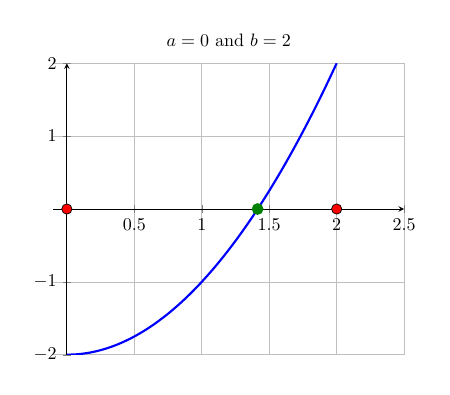
\begin{tikzpicture}[scale=0.65]
        \begin{axis}[axis lines=center, grid, domain=0:2, xmin=-0.1, xmax=2.5, ymin=-2,
            ymax=2, title={$a=0$ and $b=2$}]
            \addplot[smooth, very thick, blue] {x^2-2};
            \draw[thick, green!50!black, fill=green!50!black] (axis cs:1.414,0) circle(0.1cm);
            \draw[fill=red] (axis cs:0,0) circle(0.1cm);
            \draw[fill=red] (axis cs:2,0) circle(0.1cm);
        \end{axis}
    \end{tikzpicture}
    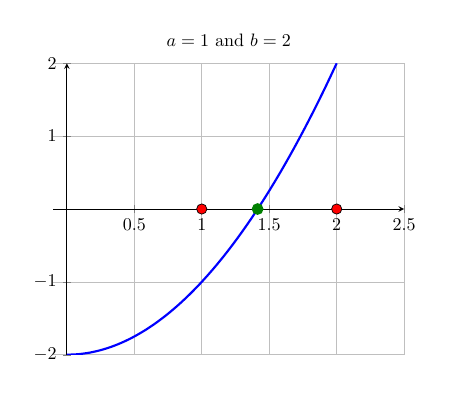
\begin{tikzpicture}[scale=0.65]
        \begin{axis}[axis lines=center, grid, domain=0:2, xmin=-0.1, xmax=2.5, ymin=-2,
            ymax=2, title={$a=1$ and $b=2$}]
            \addplot[smooth, very thick, blue] {x^2-2};
            \draw[thick, green!50!black, fill=green!50!black] (axis cs:1.414,0) circle(0.1cm);
            \draw[fill=red] (axis cs:1,0) circle(0.1cm);
            \draw[fill=red] (axis cs:2,0) circle(0.1cm);
        \end{axis}
    \end{tikzpicture}
    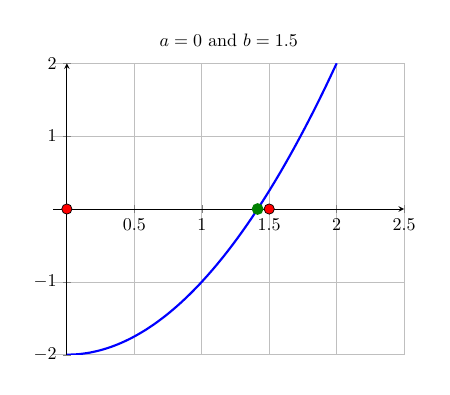
\begin{tikzpicture}[scale=0.65]
        \begin{axis}[axis lines=center, grid, domain=0:2, xmin=-0.1, xmax=2.5, ymin=-2,
            ymax=2, title={$a=0$ and $b=1.5$}]
            \addplot[smooth, very thick, blue] {x^2-2};
            \draw[thick, green!50!black, fill=green!50!black] (axis cs:1.414,0) circle(0.1cm);
            \draw[fill=red] (axis cs:0,0) circle(0.1cm);
            \draw[fill=red] (axis cs:1.5,0) circle(0.1cm);
        \end{axis}
    \end{tikzpicture}
\end{center}


\begin{problem}
    Now let's modify the Bisection Method approach.  Instead of always using the midpoint
    (which as you saw in the previous problem could take a little while to converge) let's
    draw a line between the endpoints and use the $x$-intercept as the updated guess.
    If we use this method can we improve the speed of convergence on any of the choices of
    $a$ and $b$ for this function?  Which one will now likely take the fewest steps to converge?
\begin{center}
    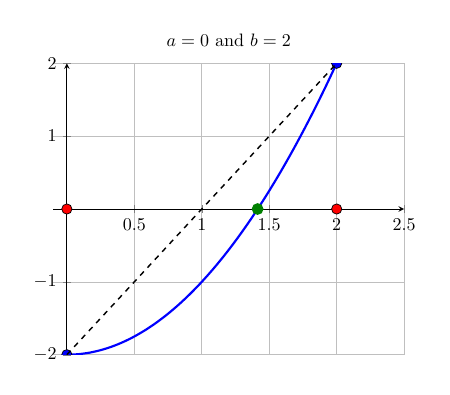
\begin{tikzpicture}[scale=0.65]
        \begin{axis}[axis lines=center, grid, domain=0:2, xmin=-0.1, xmax=2.5, ymin=-2,
            ymax=2, title={$a=0$ and $b=2$}]
            \addplot[smooth, very thick, blue] {x^2-2};
            \draw[thick, green!50!black, fill=green!50!black] (axis cs:1.414,0) circle(0.1cm);
            \draw[fill=red] (axis cs:0,0) circle(0.1cm);
            \draw[fill=blue] (axis cs:0,-2) circle(0.1cm);
            \draw[fill=red] (axis cs:2,0) circle(0.1cm);
            \draw[fill=blue] (axis cs:2,2) circle(0.1cm);
            \draw[black, thick, dashed] (axis cs:0,-2) -- (axis cs:2,2);
        \end{axis}
    \end{tikzpicture}
    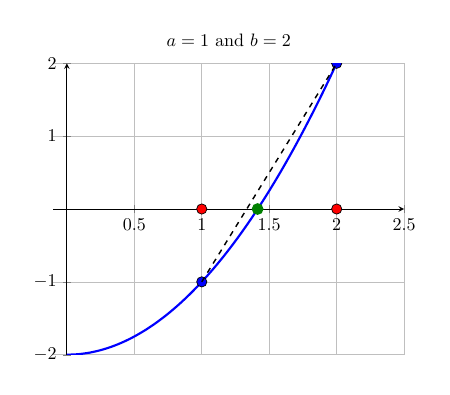
\begin{tikzpicture}[scale=0.65]
        \begin{axis}[axis lines=center, grid, domain=0:2, xmin=-0.1, xmax=2.5, ymin=-2,
            ymax=2, title={$a=1$ and $b=2$}]
            \addplot[smooth, very thick, blue] {x^2-2};
            \draw[thick, green!50!black, fill=green!50!black] (axis cs:1.414,0) circle(0.1cm);
            \draw[fill=red] (axis cs:1,0) circle(0.1cm);
            \draw[fill=blue] (axis cs:1,-1) circle(0.1cm);
            \draw[fill=red] (axis cs:2,0) circle(0.1cm);
            \draw[fill=blue] (axis cs:2,2) circle(0.1cm);
            \draw[black, thick, dashed] (axis cs:1,-1) -- (axis cs:2,2);
        \end{axis}
    \end{tikzpicture}
    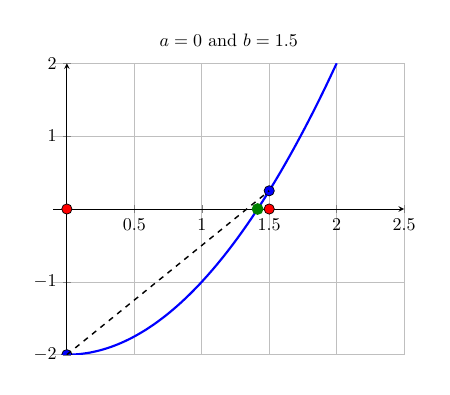
\begin{tikzpicture}[scale=0.65]
        \begin{axis}[axis lines=center, grid, domain=0:2, xmin=-0.1, xmax=2.5, ymin=-2,
            ymax=2, title={$a=0$ and $b=1.5$}]
            \addplot[smooth, very thick, blue] {x^2-2};
            \draw[thick, green!50!black, fill=green!50!black] (axis cs:1.414,0) circle(0.1cm);
            \draw[fill=red] (axis cs:0,0) circle(0.1cm);
            \draw[fill=blue] (axis cs:0,-2) circle(0.1cm);
            \draw[fill=red] (axis cs:1.5,0) circle(0.1cm);
            \draw[fill=blue] (axis cs:1.5,0.25) circle(0.1cm);
            \draw[black, thick, dashed] (axis cs:0,-2) -- (axis cs:1.5,0.25);
        \end{axis}
    \end{tikzpicture}
\end{center}
\end{problem}

The algorithm that you played with graphically in the previous problem is known as the
Regula Falsi (false position) algorithm.  It is really just a minor tweak on the Bisection
method.  After all, the algorithm is still designed to use the Intermediate Value Theorem
and to iteratively zero in on the root of the function on the given interval.

\begin{algorithm}[The Regula Falsi Method]
    Assume that $f(x)$ is continuous on the interval $[a,b]$. To make approximations of
    the solutions to the equation $f(x) = 0$, do the following:
    \begin{enumerate}
        \item Check to see if $f(a)$ and $f(b)$ have opposite signs so that the
            intermediate value theorem guarantees a root on the interval.
        \item We want to write the equation of the line connecting the points $(a,f(a))$ and
            $(b,f(b))$.
            \begin{itemize}
                \item What is the slope of this line?
                    \[ m = \underline{\hspace{1in}} \]
                \item Using the point-slope form of a line, $y-y_1 = m(x-x_1)$, what is
                    the equation of the line?
                    \[ y - \underline{\hspace{0.4in}} = \underline{\hspace{0.4in}} \cdot
                    \left( x - \underline{\hspace{0.4in}} \right) \]
            \end{itemize}
            \solution{
                \[ y - f(a) = \left( \frac{f(b) - f(a)}{b-a} \right) \left( x-a
                    \right) \]
            }
        \item Find the $x$ intercept of the linear function that you wrote in the previous
            step by setting the $y$ to zero and solving for $x$.  Call this point $x=c$.
            \[ c = \underline{\hspace{2in}} \]
            \solution{
                \[ 0 - f(a) = \left( \frac{f(b) - f(a)}{b-a} \right) \left( x-a
                    \right) \implies x = a+ \left( \frac{-f(a) (b-a)}{f(b)-f(a)} \right) \]
            }
        \item Just as we did with the bisection method, compare the signs of $f(a)$ vs
            $f(c)$ and $f(b)$ vs $f(c)$.  Replace one of the endpoints with $c$. Which one
            do you replace and why?
            \solution{Replace the endpoint where the function has the same sign as
                $f(c)$}
        \item Repeat steps 2 - 4, and stop when $f(c)$ is {\it close enough} to zero.
    \end{enumerate}
\end{algorithm}

\begin{problem}
    Draw a picture of what the Regula Falsi method does to approximate a root.
\end{problem}


\begin{problem}
    Give sketches of functions where the Regula Falsi method will perform faster than the
    Bisection method and visa versa.  Justify your thinking with several pictures and be
    prepared to defend your answers.
\end{problem}
\solution{
    The Regula Falsi method will perform very fast if the root is {\it close} to one of
    the chosen endpoints.  The bisection method will perform very vast if the root is {\it
    close} to the midoint of the two chosen endpoints.
}

\begin{problem}
    Create a new \ProgLang function called \mcode{RegulaFalsi} and write comments giving
    pseudo-code for the Regula-Falsi method.
\end{problem}

\begin{problem}
   Use your pseudo-code to create a \ProgLang function that implements the Regula Falsi method, and write a test script
   that verifies that your function works properly. Your function should accept an
    anonymous function handle as an input along with an initial lower bound, an initial
    upper bound, and an optional error tolerance. The output should be only 1 single number: the
    root.\\
    \ifnum\Python=0 \mcode{function root=RegulaFalsi(f , a , b , tol)}
    \else
    \mcode{def RegulaFalsi(f, a, b, tol):}
    \fi
\end{problem}



\newpage\section{Newton's Method}

\begin{problem}
    We are still interested in solving the equation $f(x) = 0$, but now let's leverage
    some Calculus.  In the following sequence of plots we do the following algorithm:
    \begin{itemize}
        \item Given a value of $x$ that is a decent approximation of the root, draw a
            tangent line to $f(x)$ at that point.
        \item Find where the tangent line intersects the $x$ axis.
        \item Use this intersection as the new $x$ value and repeat.
    \end{itemize}
    The first step has been shown for you.  Take a couple more steps graphically.  Does
    the algorithm appear to converge to the root?  Do you think that this will generally
    take more or fewer steps than the Bisection Method?
\begin{center}
    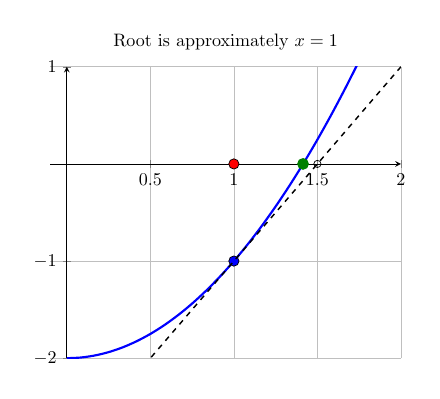
\begin{tikzpicture}[scale=0.65]
        \begin{axis}[axis lines=center, grid, domain=0:2, xmin=-0.1, xmax=2, ymin=-2,
            ymax=1, title={Root is approximately $x=1$}]
            \addplot[smooth, very thick, blue] {x^2-2};
            \draw[thick, green!50!black, fill=green!50!black] (axis cs:1.414,0) circle(0.1cm);
            \draw[fill=red] (axis cs:1,0) circle(0.1cm);
            \draw[fill=blue] (axis cs:1,-1) circle(0.1cm);
            \addplot[black, thick, dashed] {2*(x-1)-1};
            \addplot[mark=o, only marks] coordinates{(1.5,0)};
        \end{axis}
    \end{tikzpicture}
    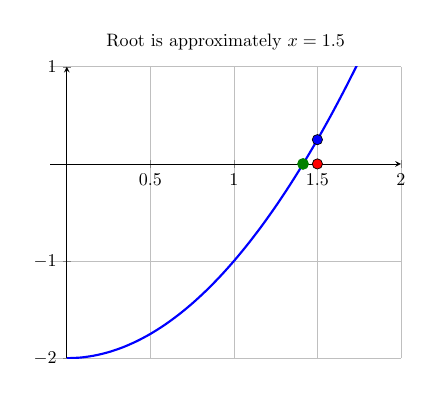
\begin{tikzpicture}[scale=0.65]
        \begin{axis}[axis lines=center, grid, domain=0:2, xmin=-0.1, xmax=2, ymin=-2,
            ymax=1, title={Root is approximately $x = 1.5$}]
            \addplot[smooth, very thick, blue] {x^2-2};
            \draw[thick, green!50!black, fill=green!50!black] (axis cs:1.414,0) circle(0.1cm);
            \draw[fill=red] (axis cs:1.5,0) circle(0.1cm);
            \draw[fill=blue] (axis cs:1.5,0.25) circle(0.1cm);
%             \addplot[black, dashed] {2*(x-1)-1};
        \end{axis}
    \end{tikzpicture}
    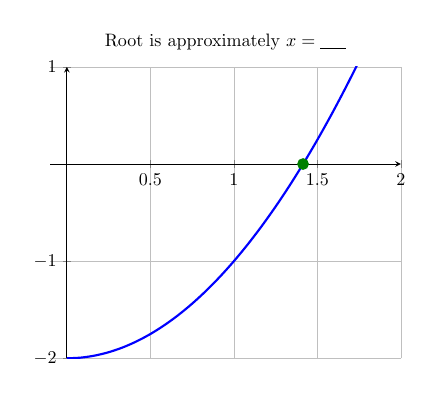
\begin{tikzpicture}[scale=0.65]
        \begin{axis}[axis lines=center, grid, domain=0:2, xmin=-0.1, xmax=2, ymin=-2,
            ymax=1, title={Root is approximately $x = \underline{\hspace{0.2in}}$}]
            \addplot[smooth, very thick, blue] {x^2-2};
            \draw[thick, green!50!black, fill=green!50!black] (axis cs:1.414,0) circle(0.1cm);
%             \draw[fill=red] (axis cs:1.5,0) circle(0.1cm);
%             \draw[fill=green] (axis cs:1.5,0.25) circle(0.1cm);
%             \addplot[black, dashed] {2*(x-1)-1};
        \end{axis}
    \end{tikzpicture}
\end{center}
\end{problem}

\begin{problem}
    If we had started at $x=0$ in the previous problem what would have happened?  Would
    this initial guess have worked to eventually approximate the root?
\end{problem}

\begin{problem}
    Make a complete list of what you must know about the function $f(x)$ for the previous
    algorithm to work?
\end{problem}

The algorithm that we just played with is known as Newton's Method.  The method was
originally proposed by Isaac Newton, and later
modified by Joseph Raphson, for solving the algebraic equation $f(x)=0$. It should be
clear that Newton's method requires the existence of the first derivative so we are asking
a bit more of our functions than we were before: In Bisection and Regula Falsi we only
asked that the functions be continuous, now we're asking that they be differentiable.  

% In very basic
% terms, this method involves iteratively finding tangent lines to a differentiable curve
% and locating where those tangent lines intersect the horizontal axis.
\begin{algorithm}[Newton's Method]
    The Newton-Raphson method for solving algebraic equations can be described as follows:
    \begin{enumerate}
        \item Check that $f$ is differentiable on a given domain and find
            a way to guarantee that $f$ has a root on that domain (this step happens by
            hand, not on the computer).
        \item Pick a starting point $x_0$ in the domain
        \item We want to write the equation of a tangent line to $f$ at the point $(x_0,
            f(x_0))$.  
            \begin{itemize}
                \item What is the slope of the tangent line to the function $f(x)$ at the
                    point $(x_0, f(x_0))$?
                    \[ m_{tangent} = \underline{\hspace{0.5in}} \]
                \item Using the point-slope form of a line, $y-y_1 = m(x-x_1)$, write the
                    equation of the tangent line to $f(x)$ at the point $(x_0, f(x_0))$.
            \[ y - \underline{\hspace{0.4in}} = \underline{\hspace{0.4in}} \cdot \left(
                x - \underline{\hspace{0.4in}} \right) \]
            \end{itemize}
            \solution{
                \[ y - f(x_0) = f'(x_0) \left( x-x_0 \right) \]
            }
        \item Find the $x$ intercept of the equation of the tangent line by setting $y=0$
            and solving for $x$.  Call this new
            point $x_1$.  
            \[ x_1 = \underline{\hspace{2in}} \]
            \solution{
                \[ x_1 = x_0 - \frac{f(x_0)}{f'(x_0)} \]
            }
        \item Now iterate the process by replacing the labels ``$x_1$'' and ``$x_0$'' in
            the previous step with $x_{n+1}$ and $x_{n}$ respectively.
            \[ x_{n+1} = \underline{\hspace{2in}} \]
            \solution{
                \[ x_{n+1} = x_{n} - \frac{f(x_n)}{f'(x_n)} \]
            }
        \item Iterate step 5 until $f(x_{n})$ is {\it close} to zero.
    \end{enumerate}
\end{algorithm}

\begin{problem}
    Draw a picture of what Newton's method does graphically.
\end{problem}


There are several ways in which Newton's Method will behave unexpectedly -- or downright
fail.  Some of these issues can be foreseen by examining the iteration formula 
\[ x_{n+1} = x_n - \frac{f(x_n)}{f'(x_n)}. \]
\begin{problem}[Failings of Newton's Method]\label{prob:newton_fail}
    There are several reasons why Newton's method could fail.  Work with your partners to
    come up with a list of all of the reasons.  Support each of your reasons with a
    sketch or an algebraic example.
\end{problem}
\solution{
    Newton's method will fail if
    \begin{itemize}
        \item the slope at the initial guess is zero (leading to no intersections of the
            tangent line with the $x$-axis), 
        \item the slope at any point in the interval is undefined,
        \item the initial guess is {\it too far away} from the intended root.
    \end{itemize}
}

\begin{problem}[An Unexpected Newton Failure]
    An interesting failure can occur with Newton's Method that you might not initially
    expect.  Consider the function $f(x) = x^3 - 2x + 2$.  This function has a root near
    $x=-1.77$.  Fill in the table below and draw the tangent lines on the figure for
    approximating the solution to $f(x) = 0$ with a starting point of $x=0$. 

    \begin{minipage}{0.5\columnwidth}
        \begin{center}
            \begin{tabular}{|c|c|c|}
                \hline
                $n$ & $x_n$ & $f(x_n)$ \\ \hline \hline
                $0$ & $0$   & $f(0) = 2$ \\ \hline
                $1$ & $0 - \frac{f(0)}{f'(0)} = 1$ & $f(1) = 1$ \\ \hline
                $2$ & $1 - \frac{f(1)}{f'(1)} =  $ & \\\hline
                $3$ & & \\\hline
                $4$ & & \\\hline
            \end{tabular}
        \end{center}
    \end{minipage}
    \begin{minipage}{0.5\columnwidth}
        \begin{center}
            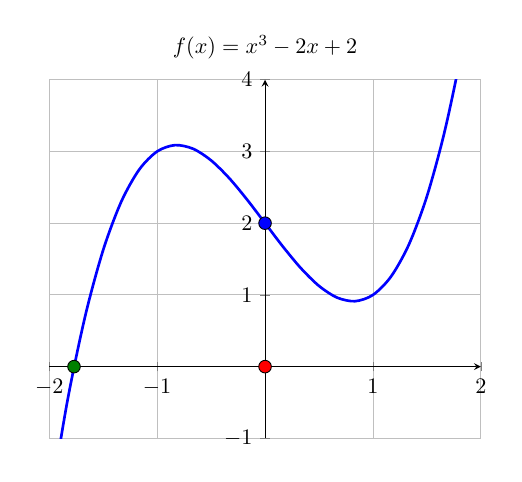
\begin{tikzpicture}[scale=0.8]
                \begin{axis}[axis lines=center, grid, xmin=-2, xmax=2, ymin=-1, ymax=4,
                    domain=-2:2, title={$f(x) = x^3 - 2x + 2$}]
                    \addplot[smooth, very thick, blue] {x^3 - 2*x + 2};
                    \draw[fill=red] (axis cs:0,0) circle(0.1cm);
                    \draw[fill=blue] (axis cs:0,2) circle(0.1cm);
                    \draw[fill=green!50!black] (axis cs:-1.77,0) circle(0.1cm);
                \end{axis}
            \end{tikzpicture}
        \end{center}
    \end{minipage}
\end{problem}

\begin{problem}[Another Unexpected Failure of Newton's Method]
    Now let's consider the function $f(x) = \sqrt[3]{x}$.  This function has a root $x=0$.
    Furthermore, it is differentiable everywhere except at $x=0$ since 
    \[ f'(x) = \frac{1}{3} x^{-2/3} = \frac{1}{3x^{2/3}}. \]
    The point of this problem is to show what can happen when the point of
    non-differentiability is precisely the point that you're looking for.  
    
    \begin{enumerate}
        \item[(a)] Fill in the
    table of iterations starting at $x=-1$, draw the tangent lines on the plot, and make a
    general observation of what is happening with the Newton iterations.

    \begin{minipage}{0.5\columnwidth}
        \begin{center}
            \begin{tabular}{|c|c|c|}
                \hline
                $n$ & $x_n$ & $f(x_n)$ \\ \hline \hline
                $0$ & $-1$   & $f(-1) = -1$ \\ \hline
                $1$ & $-1 - \frac{f(-1)}{f'(-1)} = $ &  \\ \hline
                $2$ &  & \\\hline
                $3$ & & \\\hline
                $4$ & & \\\hline
            \end{tabular}
        \end{center}
    \end{minipage}
    \begin{minipage}{0.5\columnwidth}
        \begin{center}
            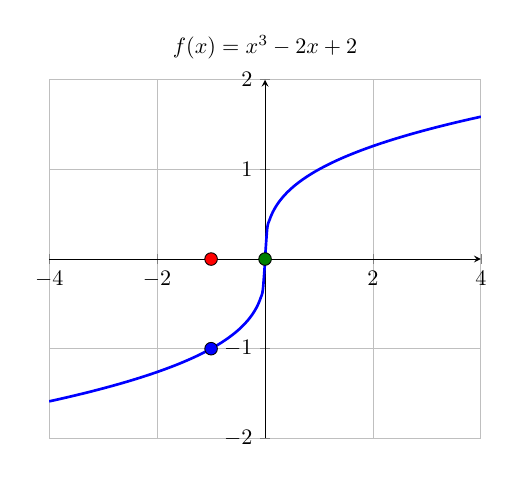
\begin{tikzpicture}[scale=0.8]
                \begin{axis}[axis lines=center, grid, xmin=-4, xmax=4, ymin=-2, ymax=2,
                    domain=-2:2, title={$f(x) = x^3 - 2x + 2$}]
                    \addplot[smooth, very thick, blue, domain=0:4, samples=100] {x^(1/3)};
                    \addplot[smooth, very thick, blue, domain=-4:0, samples=100] {-abs(x)^(1/3)};
                    \draw[fill=red] (axis cs:-1,0) circle(0.1cm);
                    \draw[fill=blue] (axis cs:-1,-1) circle(0.1cm);
                    \draw[fill=green!50!black] (axis cs:0,0) circle(0.1cm);
                \end{axis}
            \end{tikzpicture}
        \end{center}
    \end{minipage}

\item[(b)] Now let's look at the Newton iteration in a bit more detail.  Since $f(x) =
    x^{1/3}$ and $f'(x) = \frac{1}{3} x^{-2/3}$ the Newton iteration can be simplified as 
    \[ x_{n+1} = x_n - \frac{x^{1/3}}{ \left( \frac{1}{3} x^{-2/3} \right)} = x_n - 3 \frac{x^{1/3}}{x^{-2/3}} =
    x_n - 3x_n = -2x_n. \]
    What does this tell us about the Newton iterations?  \\ Hint: You should have found
    the exact same thing in the numerical experiment in part (a).
\item[(c)] Was there anything special about the starting point $x_0=-1$?  Will this
    problem exist for every starting point?
    \end{enumerate}
\end{problem}

\begin{problem}
    Create a new \ProgLang function called \mcode{Newton} and write comments giving
    pseudo-code for Newton's method.  This version of Newton's method will accept the
    function and the first derivative so you don't need to set aside any code for
    calculating the derivative.
\end{problem}

\begin{problem}
    Write a \ProgLang function for Newton's method.  Your function needs to accept an
    anonymous function handle, the derivative of $f(x)$ as an anonymous function handle,
    an initial guess, and an optional error tolerance. The only output should be the
    solution to the equation that you are solving.  Write a test script to verify that
    your Newton's method code indeed works.
    \\
    \ifnum\Python=0
    \mcode{function soln = Newton(f , df , x0 , tol)}
    \else
    \mcode{def Newton(f , df , x0 , tol):}
    \fi
\end{problem}

\begin{problem}
    The previous problem required that you calculate the derivative ahead of time for
    Newton's method.  While this is relatively easy with a computer algebra system it
    might be easier just to have your function compute the derivative for you.  Write a
    new \ProgLang function for Newton's method that accepts the function symbolically,, the initial point, and an optional error tolerance.  Your function
    must compute the derivative symbolically behind the scenes. \\
    \ifnum\Python=0
    \mcode{function soln = NewtonSymbolic(f, x0, tol)}
    \else
    \mcode{def NewtonSymbolic(f, x0, tol):}
    \fi
\end{problem}

\begin{problem}
    In Problem \ref{prob:newton_fail} you constructed several examples of where Newton's
    method will fail.  Modify your Newton's method code
    to catch these special cases and warns the user before the method fails.  Test your
    new code with several of the special cases showing that indeed you were able to catch
    them properly and give the user appropriate feedback.
\end{problem}


\begin{problem}\label{prob:newton_convergence}
    Newton's Method is known to have a {\it quadratic convergence rate}.  This means that
    there is some constant $C$ such that 
    \[ |x_{k+1} - x_*| \leq C |x_{k} - x_*|^2, \]
%     \[ \lim_{k \to \infty} \frac{|x_{k+1} - x_*|}{|x_k - x_*|^2} \]
    where $x_*$ is the root that we're hunting for.  
    To simplify the notation a bit we define $\varepsilon_{k} = |x_k - x_*|$ as the error
    in the Newton iteration at step $k$.  Therefore, there must be a constant $C$ such
    that 
    \[ \varepsilon_{k+1} \leq C \varepsilon_k^2. \]
    The quadratic convergence implies that
    if we plot the error in the new iterate on the $y$-axis and the error in the old
    iterate on the $x$ axis of a log-log plot then we will see a constant slope of 2.
    To see this we can take the log (base 10) of both sides of the previous equation to
    get 
    \[ \log(\varepsilon_{k+1}) = \log(C) + 2 \log(\varepsilon_k), \]
    and we see that this is a linear function (on a log-log plot) and the slope is 2.
    
    In this problem we're going to build a numerical experiment to verify that Newton's
    method indeed has quadratic convergence.  Modify your Newton's method code so that it
    outputs all of the iterations instead of just the final root.  Once you have the
    iterations compute the error between the approximations and the exact root. For
    simplicity let's solve the equation $x^2-2=0$.  Plot the sequence of error
    approximations with the iterate $\varepsilon_k$ on the $x$-axis and the iterate
    $\varepsilon_{k+1}$ on the
    $y$-axis of a log-log plot.  
%     \\ Your plot command will look something like: \\
%     \mcode{loglog(error(1:end-1),error(2:end),'b*')} \\where \mcode{error} is a vector
%     containing all of the errors.  
    Quadratic convergence means that at every iteration the
    error should decrease by roughly 2 orders of magnitude.  How can you see this in your
    plot?
\end{problem}


% \begin{problem}
%     Repeat the previous problem with the bisection and regula falsi
%     methods.  Plot the errors of all three methods on the same plot and discuss the rates
%     of convergence for the three methods.
% \end{problem}


\newpage\section{Quasi-Newton Methods}
Newton's method requires that you have a function and a derivative of that function.  The
conundrum here is that sometimes the derivative is cumbersome or impossible to obtain but
you still want to have the great quadratic convergence exhibited by Newton's method.

Recall that Newton's method is
\[ x_{n+1} = x_n - \frac{f(x_n)}{f'(x_n)}. \]
If we replace $f'(x_n)$ with an approximation of the derivative then we may have a method
that is {\it close} to Newton's method in terms of convergence rate but is less
troublesome to compute. Any method that replaces the derivative in Newton's method with an
approximation is called a {\bf Quasi-Newton Method}.  The first obvious way to approximate
the derivative is just to use a secant line instead of a tangent line in the Newton
iteration.  If we choose two starting points that are quite close to each other then the
slope of the secant line through those points will be approximately the same as the slope
of the tangent line.  

\begin{algorithm}[Secant Method]
    Assume that $f(x)$ is continuous and we wish to solve $f(x) = 0$ for $x$.
    \begin{enumerate}
        \item Determine if there is a root {\it near} an arbitrary starting point $x_0$.
        \item Pick a second starting point {\it near} $x_0$.  Call this second starting
            point $x_1$. Note well that the points $x_0$ and
            $x_1$ should be close to each other. (Why?)\\ (The choice here is different than for
            the Bisection  and Regula Falsi methods.)
        \item Use the backward difference 
            \[ f'(x_n) \approx \frac{f(x_n) - f(x_{n-1})}{x_n - x_{n-1}} \]
            to approximate the derivative of $f$ at $x_n$.
        \item Perform the Newton-type iteration 
            \[ x_{n+1} = x_n - \frac{f(x_n)}{ \left(  \frac{f(x_n) - f(x_{n-1})}{x_n - x_{n-1}}\right)} \]
            until $f(x_n)$ is {\it close enough} to zero.  Notice that the new iteration
            simplifies to
            \[ x_{n+1} = x_n - \frac{f(x_n)\left( x_n - x_{n-1} \right)}{f(x_n) -
            f(x_{n-1})}. \]
    \end{enumerate}
\end{algorithm}

\begin{problem}
    Draw several pictures showing what the Secant method does pictorially.
\end{problem}

\begin{problem}
    Write \ProgLang code for solving algebraic equations of the form $f(x) = 0$ with the
    Secant method.  You should ALWAYS start by writing pseudo-code as comments in your
    \ProgLang file.   Your function should accept \ifnum\Python=0 an anonymous function
    handle\else a Python function\fi, two starting
    points, and an optional error tolerance.  Also write a test script that clearly shows that your code is working.
    \\
    \ifnum\Python=0
    \mcode{function soln = SecantMethod(f, x0, x1, tol)}
    \else
    \mcode{def SecantMethod(f, x0, x1, tol):}
    \fi
\end{problem}

\begin{problem}
    Choose a non-trivial algebraic equation for which you know the solution and write a
    script to empirically determine the convergence rate of the Secant method.  You may want to
    look back at \ref{prob:newton_convergence}.
\end{problem}





\newpage\section{Exercises}

\subsection{Algorithm Summaries}
The following four problems are meant to have you re-build each of the algorithms that
we developed in this chapter.  Write all of the mathematical details completely and
clearly.  Don't just write ``how'' them method works, but give all of the mathematical
details for ``why'' it works.
\begin{problem}
    Let $f(x)$ be a continuous function on the interval $[a,b]$ where $f(a) \cdot f(b) <
    0$.  Clearly give all of the mathematical details for how the Bisection Method
    approximates the root of the function $f(x)$ in the interval $[a,b]$.  
\end{problem}

\begin{problem}
    Let $f(x)$ be a continuous function on the interval $[a,b]$ where $f(a) \cdot f(b) <
    0$.  Clearly give all of the mathematical details for how the Regula Falsi Method
    approximates the root of the function $f(x)$ in the interval $[a,b]$. 
\end{problem}

\begin{problem}
    Let $f(x)$ be a differentiable function with a root {\it near} $x=x_0$.  Clearly give
    all of the mathematical details for how Newton's Method approximates the root of the
    function $f(x)$.
\end{problem}

\begin{problem}
    Let $f(x)$ be a continuous function with a root {\it near} $x=x_0$.  Clearly give
    all of the mathematical details for how the Secant Method approximates the root of the
    function $f(x)$.
\end{problem}

\subsection{Applying What You've Learned}

\begin{problem}
    In this problem you will demonstrate that all of your root finding codes work.
    At the beginning of this chapter we proposed the algebraic equation solving problem
    \[ 3\sin(x) + 9 = x^2 - \cos(x). \]
    Write a \ProgLang script that calls upon your Bisection, Regula Falsi, Newton, and
    Secant, methods one at a time to find the positive solution to this equation.  Your
    script needs to output the solutions in a clear and readable way so you can tell which
    answer can from which root finding algorithm. Clearly all of your root finding
    routines will be stored as \ProgLang functions so be sure to turn in all of these
    functions along with this problem.
\end{problem}

\begin{problem}[Order of Convergence]
    A root-finding method has a convergence rate of order $M$ if there is a constant $C$
    such that 
    \[ |x_{k+1} - x_*| \leq C |x_k - x_*|^M. \]
%     \[ \frac{|x_{k+1} - x_*|}{|x_k - x_*|^M} \]
    Here, $x_*$ is the exact root, $x_k$ is
    the $k^{th}$ iteration of the root finding technique, and $x_{k+1}$ is the
    $(k+1)^{st}$ iteration of the root finding technique.  We will call the value
    $\varepsilon_k = |x_{k}-x_*|$ the ``old'' error since it is the error in the method at the old step.
    We will call the value $\varepsilon_{k+1} = |x_{k+1}-x_*|$ the ``new'' error since it is the error in the
    method at the new step.
    \begin{enumerate}
        \item[(a)] If we consider the equation 
            \[ |x_{k+1} - x_*| \leq C |x_k - x_*|^M \]
            and take the logarithm (base 10) of both sides then we get
            \[ \log\left( |x_{k+1} - x_*| \right) \leq \underline{\hspace{1in}} +
            \underline{\hspace{1in}} \]
        \item[(b)] In part (a) you should have found that the log of new error is a linear
            function of the log of the old error.  What is the slope of this linear
            function on a log-log plot?
        \item[(c)] In the plots below you will see three different log-log plots of the new
            error to the old error for different root finding techniques.  What is the
            order of the convergence rate for each of these methods?
        \item[(d)] In your own words, what does it mean for a root finding method to have
            a ``first order convergence rate''?  ``Second order convergence rate''? etc.
    \end{enumerate}
\begin{center}
    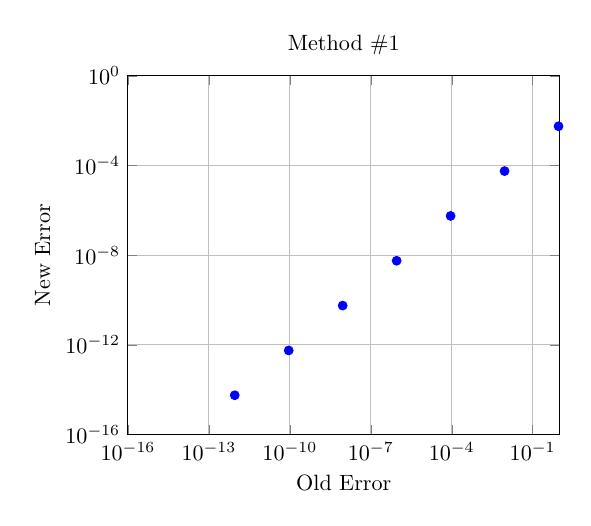
\begin{tikzpicture}[scale=0.8]
        \begin{loglogaxis}[grid, xmin=1e-16, xmax=1, ymin=1e-16, ymax=1, title={Method
            \#1}, xlabel={Old Error}, ylabel={New Error}]
            \addplot[only marks, color=blue] coordinates{
                (	0.909538969	,	0.005632421	)
                (	0.00909539	,	5.63242E-05	)
                (	9.09539E-05	,	5.63242E-07	)
                (	9.09539E-07	,	5.63242E-09	)
                (	9.09539E-09	,	5.63242E-11	)
                (	9.09539E-11	,	5.63242E-13	)
                (	9.09539E-13	,	5.63242E-15	)
                (	9.09539E-15	,	5.63242E-17	)                    
            };
        \end{loglogaxis}
    \end{tikzpicture}
    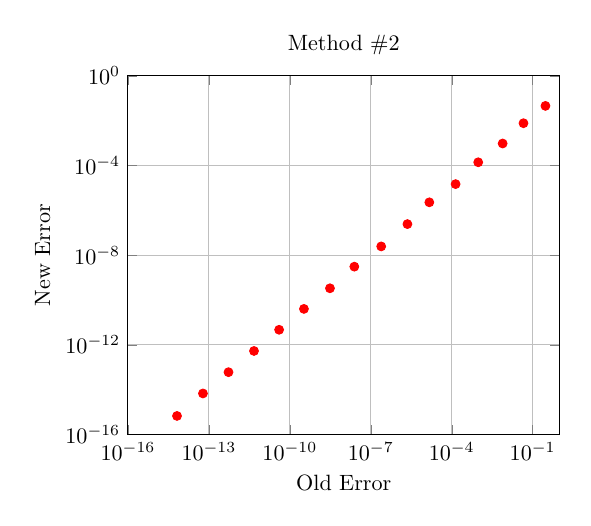
\begin{tikzpicture}[scale=0.8]
        \begin{loglogaxis}[grid, xmin=1e-16, xmax=1, ymin=1e-16, ymax=1, title={Method
            \#2}, xlabel={Old Error}, ylabel={New Error}]
            \addplot[only marks, color=red] coordinates{
                (	0.297389258	,	0.04564068	)
                (	0.04564068	,	0.007707808	)
                (	0.007707808	,	0.000959205	)
                (	0.000959205	,	0.000139301	)
                (	0.000139301	,	1.48093e-05	)
                (	1.48093e-05	,	2.27993e-06	)
                (	2.27993e-06	,	2.43575e-07	)
                (	2.43575e-07	,	2.45946e-08	)
                (	2.45946e-08	,	3.07365e-09	)
                (	3.07365e-09	,	3.33233e-10	)
                (	3.33233e-10	,	4.01008e-11	)
                (	4.01008e-11	,	4.70157e-12	)
                (	4.70157e-12	,	5.33293e-13	)
                (	5.33293e-13	,	6.03244e-14	)
                (	6.03244e-14	,	6.782e-15	)                    
                (6.5853e-15,	6.73173e-16)
                (6.73173e-16,	7.63516e-17)
            };
        \end{loglogaxis}
    \end{tikzpicture}
    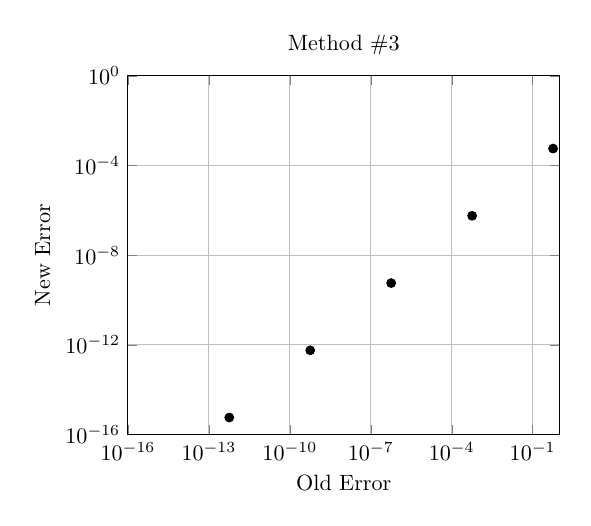
\begin{tikzpicture}[scale=0.8]
        \begin{loglogaxis}[grid, xmin=1e-16, xmax=1, ymin=1e-16, ymax=1, title={Method
            \#3}, xlabel={Old Error}, ylabel={New Error}]
            \addplot[only marks, color=black] coordinates{
(	0.570332325	,	0.000570332	)
(	0.000570332	,	5.70332E-07	)
(	5.70332E-07	,	5.70332E-10	)
(	5.70332E-10	,	5.70332E-13	)
(	5.70332E-13	,	5.70332E-16	)
(	5.70332E-16	,	5.70332E-19	)                
            };
        \end{loglogaxis}
    \end{tikzpicture}
\end{center}

\end{problem}


\begin{problem}
    \begin{enumerate}
        \item[(a)] Write code and create plots to demonstrate that the Bisection Method
            has approximately first order convergence.  Demonstrate this result on several
            differen equation-solving problems.
        \item[(b)] Write code and create plots to demonstrate that Newton's Method has
            second order convergence.  Demonstrate this result on the same
            equation-solving problems from part (a).
    \end{enumerate}
\end{problem}

\begin{problem}
    Multiple Choice: For every step of Newton's method the new estimate of the error
    between the Newton iteration and the exact answer is approximately:
    \begin{enumerate}
        \item[(a)] the same as it was on the previous step.
        \item[(b)] ten times smaller than it was on the previous step
        \item[(c)] one hundred times smaller than it was on the previous step
        \item[(d)] one thousand times smaller than it was on the previous step
    \end{enumerate}
    Defend your answer with a sentence or two.
\end{problem}


% \begin{problem}
%     Bob solved the equation $f(x) = 0$ for a differentiable function using two different
%     methods studied in this chapter.  He
%     happened to know the root for the function $f(x)$ so he build a vector of absolute
%     errors for each of the two methods.  In Figure \ldots you see the error at the
%     $n^{th}$ iteration on the horizontal axis and the error at the $(n+1)^{st}$ iteration
%     on the vertical axis. From this plot what can you say about the method in  
% \end{problem}
\begin{problem}
    Write \ProgLang code that produces a loglog plot that compares the convergence rates for
    the bisection method, the regula-falsi method, Newton's method, and the secant method
    on a problem where we know the exact answer. 
\end{problem}


\begin{problem}
    Show several plots that demonstrates that the Chebyshev Method,
    \[ x_{n+1} = x_n - \frac{f(x_n)}{f'(x_n)} - \frac{1}{2} \left( \frac{f(x_n)}{f'(x_n)}
    \right)^2 \frac{f''(x_n)}{f'(x_n)}, \]
    exhibits a third-order convergence rate. That is, create a log-log plot of the
    successive errors for several different equation-solving problems.  What does this
    ``third order convergence'' mean about the successive
    approximations in the Chebyshev iterations?  What are the pro's and con's to using
    Chebyshev's method instead of Newton's method?
\end{problem}





\begin{problem}
    Compare the number of iterations necessary for convergence to within $10^{-8}$ for
    both the bisection method and the regula falsi method on several test problems. Find
    example problems where bisection converges faster and examples where regula falsi
    converges faster. Write a test script that clearly indicates to the user which
    equation was being solved, which endpoints were used, and which root finding technique
    performed faster.
\end{problem}

\begin{problem}
    An object falling vertically through the air is subject to friction due to air
    resistance as well as gravity.  The function describing the position of such a
    function is 
    \[ s(t) = s_0 - \frac{mg}{k} t + \frac{m^2 g}{k^2}\left( 1- e^{-kt/m} \right), \]
    where $m$ is the mass measured in kg, $g$ is gravity measured in meters per second per
    second, $s_0$ is the
    initial position measured in meters, and $k$ is the
    coefficient of air resistance.
    \begin{enumerate}
        \item[(a)] What are the units of the parameter $k$?
        \item[(b)] If $m = 1$kg, $g=9.8$m/s$^2$, $k=0.1$, and $s_0 = 100$m how long will it take
            for the object to hit the ground?  Find your answer to within 0.01 seconds.
        \item[(c)] The value of $k$ depends on the aerodynamics of the object and might be
            challenging to measure.  We want to perform a sensitivity analysis on your
            answer to part (b) subject to small measurement errors in $k$.  If the value
            of $k$ is only known to within 10\% then what are your estimates of when the
            object will hit the ground?
    \end{enumerate}
\end{problem}


\begin{problem}[Modified from \cite{Chartier}]
    An artillery officer wishes to fire his cannon on an enemy brigade.  He wants to know
    the angle to aim the cannon in order to strike the target.  Follow the steps below to
    arrive at an approximate answer.
    \begin{enumerate}
        \item[(a)] Solve the simple differential equation $v_y'(t) = -g$ by hand where $v_y(t)$
            is the vertical velocity of the canon and gravity is given as $g \approx
            9.8$m/s$^2$.  We don't know the initial velocity so just use $v(0) = v_0$ and
            hence $v_y(0) = v_0 \sin(\theta)$. Note: your answer will have a ``$v_0$'' and a
            ``$\sin(\theta)$'' in it.
        \item[(b)] Solve the differential equation $s_y'(t) = v_y(t)$ by hand for the position
            function $s_y(t)$.  Assume that $s_y(0) = 0$.  Your answer will still have a ``$v_0$'' and a
            ``$\sin(\theta)$'' in it.
        \item[(c)] Solve $s_y(t) = 0$ by hand for $t$ in terms of $v_0$ and $\theta$ to
            find a function for the amount of time the projectile takes to reach the
            ground.
        \item[(d)] In the absence of air resistance the projectile will have a constant
            velocity in the horizontal direction.  Solve the differential equation
            $s_x'(t) = v_0 \cos(\theta)$ for the horizontal position function $s_x(t)$.  
        \item[(e)] The range function $R(v_0,\theta)$ can be found by substituting the
            time from part (c) into the horizontal position function in part (d).  Find
            the function $R(v_0,\theta)$.
        \item[(f)] For a certain projectile and canon the initial velocity is $v_0 =
            126$m/s.  We want to give the artillery officer a distance, $d$, and have them
            calculate the angle to hit the target.  Write \ProgLang code to approximate
            $\theta$ in the equation 
            \[ R(126,\theta) = d. \]
            (Hint: remember that we can rewrite the equation $R(126,\theta)=d$ in the form
            $f(\theta) = 0$ for some function $f$ so that we can actually use our
            numerical root finding techniques. See the discussion at the very beginning of
            this chapter.)

            Report a table of values of the form shown below and provide an appropriate
            plot showing your results.  Clearly some distances will be out of range so be
            sure to clearly indicate the range of the weapon.
            \begin{center}
                \begin{tabular}{|c|c|}
                    \hline
                    Distance ($d$ meters) & Angle ($\theta$) \\ \hline \hline
                    0 & \\
                    25 & \\
                    50 & \\
                    100 & \\
                    $\vdots$ & \\ \hline
                \end{tabular}
            \end{center}
    \end{enumerate}
\end{problem}
\hint{
    Remember that solving the equation $R(126,\theta) = d$ is the same as solving the
    equation $R(126,\theta)-d = 0$.  This is the setup you need for all of our root
    finding techniques.
}


\begin{problem}
    Consider our four primary root finding methods: Bisection, Regula Falsi, Newton's method, and the
    Secant method.  
    \begin{enumerate}
        \item[(a)] For each method give a mathematical situation where you might want to
            use the method and give a mathematical situation where you might not want to
            use the method.  
        \item[(b)] For each of these methods give one example where the method will fail.  
        \end{enumerate}
        Support your arguments with proper mathematics.  You are welcome to argue
        graphically but be sure to fully explain your graphical reasoning.
\end{problem}




\begin{problem}
    In Single Variable Calculus you studied methods for finding local and global extrema
    of functions. You likely recall that part of the process is to set the first
    derivative to zero and to solve for the independent variable (remind yourself why
    you're doing this).  The trouble with this process is that it may be very very
    challenging to do the algebraic solve by hand.  This is a perfect place for Newton's
    method or any other root finding techinque! \\
    Find the local extrema for the function $f(x) = x^3(x-3)(x-6)^4$ and explicitly
    demonstrate, without the use of a plot, that you have found all of the local extrema.
\end{problem}
\hint{
    Recall that if the derivative of a single variable function is zero then the function
    has a possible local extrema.  In this problem it is likely best to find the first and
    second derivatives on paper before writing any code.
}



\begin{problem}

    A {\it fixed point} of a function $f(x)$ is a point that solves the equation $f(x) =
    x$.  Fixed points are interesting in iterative processes since fixed points don't
    change under repeated application of the function $f$.  

    For example, consider the function $f(x) = x^2 - 6$.  The fixed points of $f(x)$ can be found by
    solving the equation $x^2 - 6 = x$ which, when simplified algebraically, is $x^2 - x -
    6 = 0$.  Factoring the left-hand side gives $(x-3)(x+2)=0$ which implies that $x=3$
    and $x=-2$ are fixed points for this function. That is, $f(3) = 3$ and $f(-2) = -2$.
    Notice, however, that finding fixed points is identical to a root finding problem.
    \begin{enumerate}
        \item[(a)] Use a numerical root-finding algorithm to find the fixed points of the
            function $f(x) = x^2 - 6$ on the interval $[0,\infty)$.
            \item[(b)] Find the fixed points of the function $f(x) =
                \sqrt{\frac{8}{x+6}}$.
        \end{enumerate}
    \end{problem}



\newpage\section{Projects}
In this section we propose several ideas for projects related to numerical algebra.  These
projects are meant to be open ended, to encourage creative mathematics, to push your
coding skills, and to require you to write and communicate your mathematics.  Take the
time to read Appendix \ref{app:writing_projects} before you write your final solution.

\subsection{Basins of Attraction}

Let $f(x)$ be a differentiable function with several roots.  Given a starting $x$
value we should be able to apply Newton's Method to that starting point and we will
converge to one of the roots (so long as you aren't in one of the special cases
discussed earlier in the chapter).  It stands to reason that starting points {\it
near} each other should all end up at the same root, and for some functions this is
true.  However, it is not true in general.  

A {\bf basin of attraction} for a root is the set of $x$ values that converges to that
root under Newton iterations.  In this problem you will produce colored plots showing
the basins of attraction for all of the following functions.  Do this as follows:
\begin{itemize}
    \item Find the actual roots of the function by hand (this should be easy on the
        functions below).  
    \item Assign each of the roots a different color.
    \item Pick a starting point on the $x$ axis and use it to start Newton's Method.
    \item Color the starting point according to the root that it converges to.
    \item Repeat this process for many many starting points so you get a colored
        picture of the $x$ axis showing where the starting points converge to.
\end{itemize}
The set of points that are all the same color are called the {\bf basin of attraction}
for the root associated with that color.

\begin{enumerate}
    \item[(a)] $f(x) = (x-4)(x+1)$
    \item[(b)] $g(x) = (x-1)(x+3)$
    \item[(c)] $h(x) = (x-4)(x-1)(x+3)$
    \item[(d)] Find a single-variable function of your own that has an interesting
        picture of the basins of attraction.
    \item[(e)] Now for the fun part!  Consider the function $f(z) = z^3 - 1$ where $z$
        is a complex variable.  That is, $z = x + iy$ where $i = \sqrt{-1}$.  From the
        Fundamental Theorem of Algebra we know that there are three roots to this
        polynomial in the complex plane.  In fact, we know that the roots are $z_0 =
        1$, $z_1 = \frac{1}{2}\left( -1 + \sqrt{3} i \right)$, and $z_2 =
        \frac{1}{2} \left( -1 - \sqrt{3} i \right)$ (you should stop now and check
        that these three numbers are indeed roots of the polynomial $f(z)$).  Your job
        is to build a picture of the basins of attraction for the three roots in the
        complex plane.  This picture will naturally be two-dimensional since numbers
        in the complex plane are two dimensional (each has a real and an imaginary
        part).  When you have your picture give a thorough write up of what you found.
    \item[(f)] Now pick your favorite complex-valued function and build a picture of
        the basins of attraction.  Consider this an art project!  See if you can come
        up with the prettiest basin of attraction picture.
\end{enumerate}






